\chapter{Numerical implementation}\label{chap:Numerical}

In this modern era of fission theory which is dependent upon high-performance computers, it is worth discussing some of the numerical and computational issues associated with computing the potential energy surface, the collective inertia, and the collective dynamics of a fissioning nucleus.

\section{Calculating the potential energy surface}
By far, the most time-consuming part of a microscopic fission calculation is computing the PES. For this we use a pair of DFT solvers, HFODD~\cite{Schunck2017} and HFBTHO~\cite{Perez2017}, which solve the HFB equations in a deformed harmonic oscillator basis. The solver HFBTHO is limited to shapes with axial symmetry, while HFODD allows for the breaking of any symmetry needed (for instance, rotational invariance or parity). Since the major bottleneck of each of these programs involves constructing matrices which represent nucleonic densities and currents and then diagonalizing the HFB Hamiltonian matrix, the flexibility of symmetry breaking drastically increases the time-to-solution. Thus, HFBTHO is used for fast calculations, while HFODD is slower but more flexible.

Fortunately, the problem of calculating a PES is embarrassingly-parallel. So while an individual point in the PES may be time-consuming to compute, many points can be computed on a large platform with many processors simultaneously. This does have its limitations; highly-deformed configurations may be unstable or ill-defined. In such cases, one fix can sometimes be to use a nearby point which converged successfully as a seed function.

%Certain parts of the procedure can be parallelized using shared-memory parallelism, such as QMULCM, which does what again? It readjusts the Lagrange parameters of the constraints based on the perturbative approximation fot he QRPA matrix.

\subsection{PES Tools}
Apart from the issue of walltime, generating a PES creates a lot of data, which quickly becomes unwieldy. To help manage all this data, a Python module called PES Tools was developed for manipulating, extracting, interpolating, and plotting~\cite{PES_tools}. Aside from the parser scripts, which collect data from the output of a particular DFT solver and store it in an XML data structure, PES Tools is not dependent on a specific DFT solver.

In particular, a submodule was created to interface between PES Tools and Fission Tools~\cite{fission_tools}, a set of codes used for fission calculations. These codes are described in the following sections.

\section{Calculating the collective inertia}\label{sect:M_numerical}
The partial derivatives from equation~\eqref{eq:mATDHFB-np} are computed using the Lagrange three-point formula~\cite{Baran2011}:

\begin{equation}\label{eq:finite-diffs}
\left(\frac{\partial \mathcal{R}}{\partial q}\right)_{q=q_0} \approx 
    \frac{-\delta q'}{\delta q \left(\delta q + \delta q'\right)}\mathcal{R}(q_0-\delta q) + 
    \frac{\delta q - \delta q'}{\delta q \delta q'}\mathcal{R}(q_0) + 
    \frac{\delta q}{\delta q' \left(\delta q + \delta q'\right)}\mathcal{R}(q_0+\delta q') .
\end{equation}

\noindent The accuracy and precision of the collective inertia $\mathcal{M}$ are therefore functions of the spacings $\delta q$ and $\delta q'$, and of $\mathcal{R}$. An accurate value of the collective inertia is especially important for computing half-lives, for which there is an exponential dependence on $\mathcal{M}$.

\begin{figure}
	\centering
	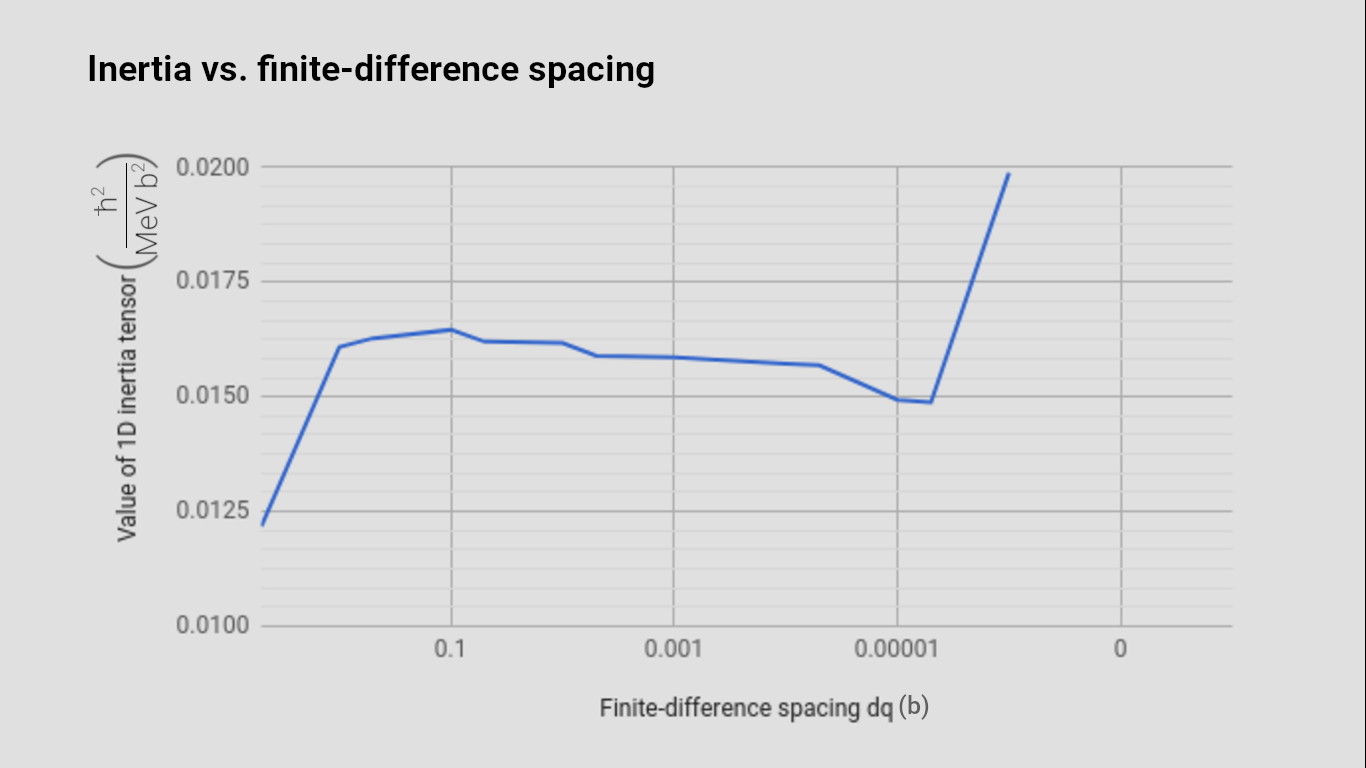
\includegraphics[width=0.7\linewidth]{TeX_files/Num-dq_spacing}
	\caption[$\mathcal{M}_{q20q20}$ calculated for some configuration of $^{240}$Pu as a function of finite-difference spacing $\delta q$.]{$\mathcal{M}_{q20q20}$ calculated for some configuration of $^{240}$Pu as a function of finite-difference spacing $\delta q$.}
	\label{fig:num-dqspacing}
\end{figure}

Finite-difference calculations such as~\eqref{eq:finite-diffs} are dependent on the size of the finite-difference spacing $\delta q$. Figure~\ref{fig:num-dqspacing} shows the effect of different values of $\delta q (= \delta q')$ on the collective inertia for some configuration of $^{240}$Pu. After some initial fluctuations for large $\delta q$, the value of $\mathcal{M}$ appears to be nearly constant over a range of several values of $\delta q$. The abrupt jump at the end of Figure~\ref{fig:num-dqspacing} is related to the level of convergence of the density matrix $\mathcal{R}$, illustrated in Figure~\ref{fig:num-rhoconv}.

\begin{figure}
	\centering
	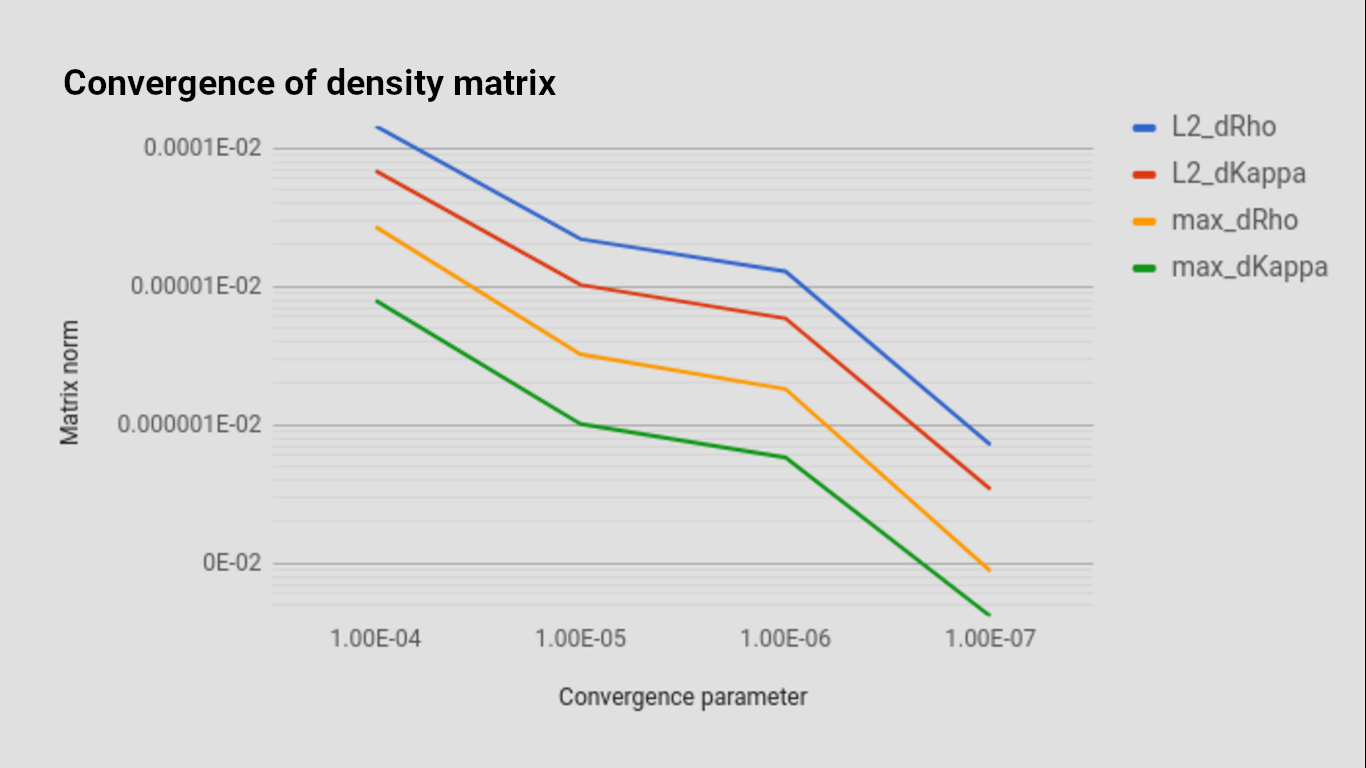
\includegraphics[width=0.7\linewidth]{TeX_files/Num-rho_conv}
	\caption[Norm of the difference matrix between subsequent iterations of the density]{Norm of the difference matrix between subsequent iterations of the density.}
	\label{fig:num-rhoconv}
\end{figure}

Figure~\ref{fig:num-rhoconv} shows the norm of the matrix which corresponds to the difference between the density matrix at the last iteration and the second-to-last iteration. This can be thought of as numerical noise. Predictably, the noise decreases as the convergence parameter becomes tighter. This gives a sense of the uncertainty $\delta \mathcal{R}$ associated with $\mathcal{R}$, which in turn should be propagated through equations~\eqref{eq:finite-diffs} and~\eqref{eq:mATDHFB-np}. Additionally, if the amount of noise in $\mathcal{R}$ is much larger than, or comparable in size to $\delta q$, then $\mathcal{M}$ will suffer from jumps like the one near $\delta q \approx 10^{-6}$ in Figure~\ref{fig:num-dqspacing}. To avoid such problems in our calculations, our finite-difference spacing $\delta q$ should be larger than our HFB convergence parameter.

There are additional complications which arise in the finite-temperature formalism. These are discussed in Appendix~\ref{append:TD-ATDHFB}.

\section{Minimum action path}
For the tunneling part of the collective evolution described in Section~\ref{sect:wkb}, the dynamic programming method~\cite{Baran1981} was used to minimize the action. The dynamic programming method proceeds inductively: once the minimum action is known for all grid points up to a certain value of $Q_{20}$, say $q_{20}^n$, then the minimum action at each grid point in the $(n+1)$th layer with $Q_{20}=q_{20}^{n+1}$ is obtained by computing the action between each grid point in layer $n$ and each grid point in layer $n+1$, and then selecting the path which minimizes the total action at each grid point in layer $n+1$:

\begin{equation}
\left.S_{min}(\vec{Q})\right|_{Q_{20}=q_{20}^{n+1}} = \mathrm{argmin}_{\vec{Q'}}\left.\left(S_{min}(\vec{Q'}) + \Delta S_{min}(\vec{Q},\vec{Q'})\right)\right|_{Q'_{20}=q_{20}^{n}, Q_{20}=q_{20}^{n+1}}.
\end{equation}

The inductive step which connects layers $n$ and $n+1$ involves several small, independent calculations which lend themselves well to shared-memory parallelism. This was implemented in the code using OpenMP, resulting in a walltime reduction from order $\mathcal{O}(n^D)$ to $\mathcal{O}(n^D/m)$, where $m$ is the number of processors (with the usual caveats that parallelization requires additional overhead time, and that the actual speedup might be somewhat less when the number of processors $m$ reaches the same order as the number of points per layer, $n^{D-1}$). In a 2D calculation, where the runtime is on the order of seconds, the difference is inconsequential. However, this speedup was essential for the analysis of a 4D PES, as described in Chapter~\ref{chap:294Og}.


\section{Stochastic Langevin calculations}
Once the action and relative probability are known for a set of points along the outer turning line, Langevin trajectories are computed starting from each outer turning point. These are straightforwardly evaluated at discrete time steps over a discretized PES mesh.

Because of the random force term in equation~\eqref{eq:langevin}, a large number of trajectories per outer turning point must be computed to reduce statistical uncertainty. Fortunately, each trajectory is completely independent of every other trajectory, lending the code readily to shared-memory parallelism. However, for the Fission Tools Langevin code, distributed-memory parallelism was chosen over shared-memory parallelism in order to simplify access to shared resources, such as variables and output files.